\section{Funcões de Várias Variáveis}



\subsection*{Definição}
\begin{frame}[label=funcoes]
\frametitle{Funções de Várias Variáveis }
%\begin{scriptsize}

\uncover<1->{ Uma \dt{função real $f$ de $n$ variáveis} é uma relação que associa a cada n-upla $(x_1,\ldots,x_n)\in D\subset \R^n$ um único  número real $z=f(x_1,\ldots,x_n)$. O subconjunto $D$ de $\R^n$ é chamado \dt{domínio} da função $f$. Podemos denotar a função $f$ por
\[\begin{array}{ccl}
f:& D\subset\R^n & \longrightarrow \R\\
& (x_1,\ldots,x_n) & \longmapsto z=f(x_1,\ldots,x_n)
\end{array}\]
 }

\begin{center}
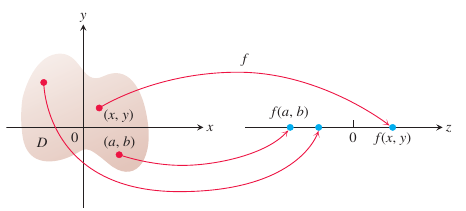
\includegraphics[scale=.7]{figuras/func.png}
\end{center}

%\end{scriptsize}
\end{frame}

\begin{frame}[label=funcoes]

\begin{exe} \begin{enumerate}
\item A função $V(r,h)=\pi r^2h$, $r,h>0$ é uma função de duas variáveis que  fornece o volume de um cilindro circular reto de raio da base $r$ e altura $h$.

 \item A função $z=f(x,y)=\frac{1}{x-y}$ é uma função de duas variáveis cujo domínio são todos os pontos $(x,y)\in \R^2$ tais que $x\neq y$.
 
 \item A função $\dps f(x,y,z)=\frac{1}{(x^2+y^2+z^2)^{3/2}}$ é uma função de três variáveis cujo domínio são todos os pontos $(x,y,z)\in \R^3$ tais que $x^2+y^2+z^2\neq 0$, ou seja, $\R^3\setminus\{0\}$.
 \end{enumerate}
 \end{exe}
 
\end{frame}


\subsection*{Gráfico de função de duas variáveis}
\begin{frame}[label=funcoes]{Gráfico de uma função de duas variáveis}
%\begin{scriptsize}

O \dt{gráfico de uma função} $f:D\subset \R^2\to \R$, denotado por $G_f$, é o subconjunto do $\R^{3}$ formado por todos os pontos  da forma $(x,y,f(x,y))$, isto é,
\[G_f:=\{(x,y,z)\in \R^{3};\ z=f(x,y),\ (x,y)\in \R^2\}\] 

\begin{center}
	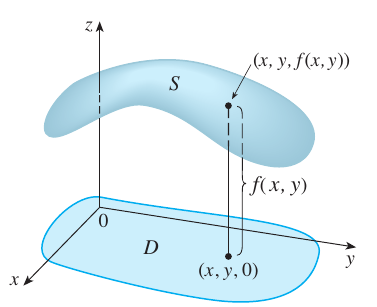
\includegraphics[scale=0.5]{figuras/grafico-f.png}
\end{center}



%\uncover<1->{\begin{exe} A temperatura em cada ponto $(x,y)$ de uma placa de metal plana é dada, em graus, pela função $T(x,y)=9x^2+4y^2$.
%\begin{enumerate}[a)]
%\item Encontre a temperatura no ponto $(1,2)$.
%\item Encontre a equação da curva ao longo da qual a temperatura tem um valor constante e igual a 36 graus.
%\item Esboce a curva do item anterior.
%\end{enumerate}
%\end{exe}}

%\end{scriptsize}
\end{frame}


\begin{frame}[label=funcoes]
	
	\begin{block}{Temperatura abaixo da superfície da Terra}
 A temperatura ${\color{red}w}$ abaixo da superfície da Terra é uma função da profundidade $x$ abaixo da superfície e da época do ano $t$. Se medirmos ${\color{blue}x}$ em pés e ${\color{blue}t}$ como o número de dias decorridos a partir da data esperada da maior temperatura anual da superfície, podemos modelar a variação da temperatura com a função
 \[{\color{red}w}=\cos(1.7\times 10^{-2}{\color{blue}t}-0.2 {\color{blue}x})e^{-0.2 {\color{blue}x}}\]
	\end{block}
	
	

\begin{center}
	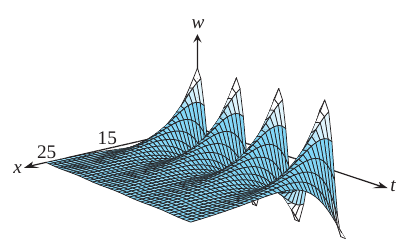
\includegraphics[scale=0.5]{figuras/grafico-2.png}
\end{center}
	
\end{frame}

\begin{frame}[label=funcoes]
\begin{exe}
	Esboce o gráfico da função  $f(x,y)=6-3x-2y$.
\end{exe}
\end{frame}

\begin{frame}[label=funcoes, fragile=singleslide]
\begin{block}{ }
\begin{scriptsize}
\begin{pyverbatim}
import matplotlib.pyplot as plt
import numpy as np

def f(x, y):
    return 6-3*x-2*y

x =y=np.linspace(-5,5, 25)

X,Y=np.meshgrid(x, y)
Z = f(X, Y)

fig=plt.figure()
ax=plt.axes(projection='3d')

ax.set_xlabel('x')
ax.set_ylabel('y')
ax.set_zlabel('z')
ax.plot_surface(X, Y, Z,cmap='viridis')

plt.show()
\end{pyverbatim}
\end{scriptsize}
\end{block}



\end{frame}

\begin{frame}[label=funcoes,fragile=singleslide]
\begin{pycode}
import matplotlib.pyplot as plt
import numpy as np

def f(x, y):
    return 6-3*x-2*y

x =y= np.linspace(-5,5, 25)

X, Y = np.meshgrid(x, y)
Z = f(X, Y)

fig = plt.figure()
ax = plt.axes(projection='3d')
ax.view_init(elev=30, azim=30, roll=0)

ax.set_xlabel('x')
ax.set_ylabel('y')
ax.set_zlabel('z')
ax.plot_surface(X, Y, Z,cmap='viridis')


plt.savefig('figuras/grafico1.png',transparent=False,dpi=400)
\end{pycode}

\begin{center}
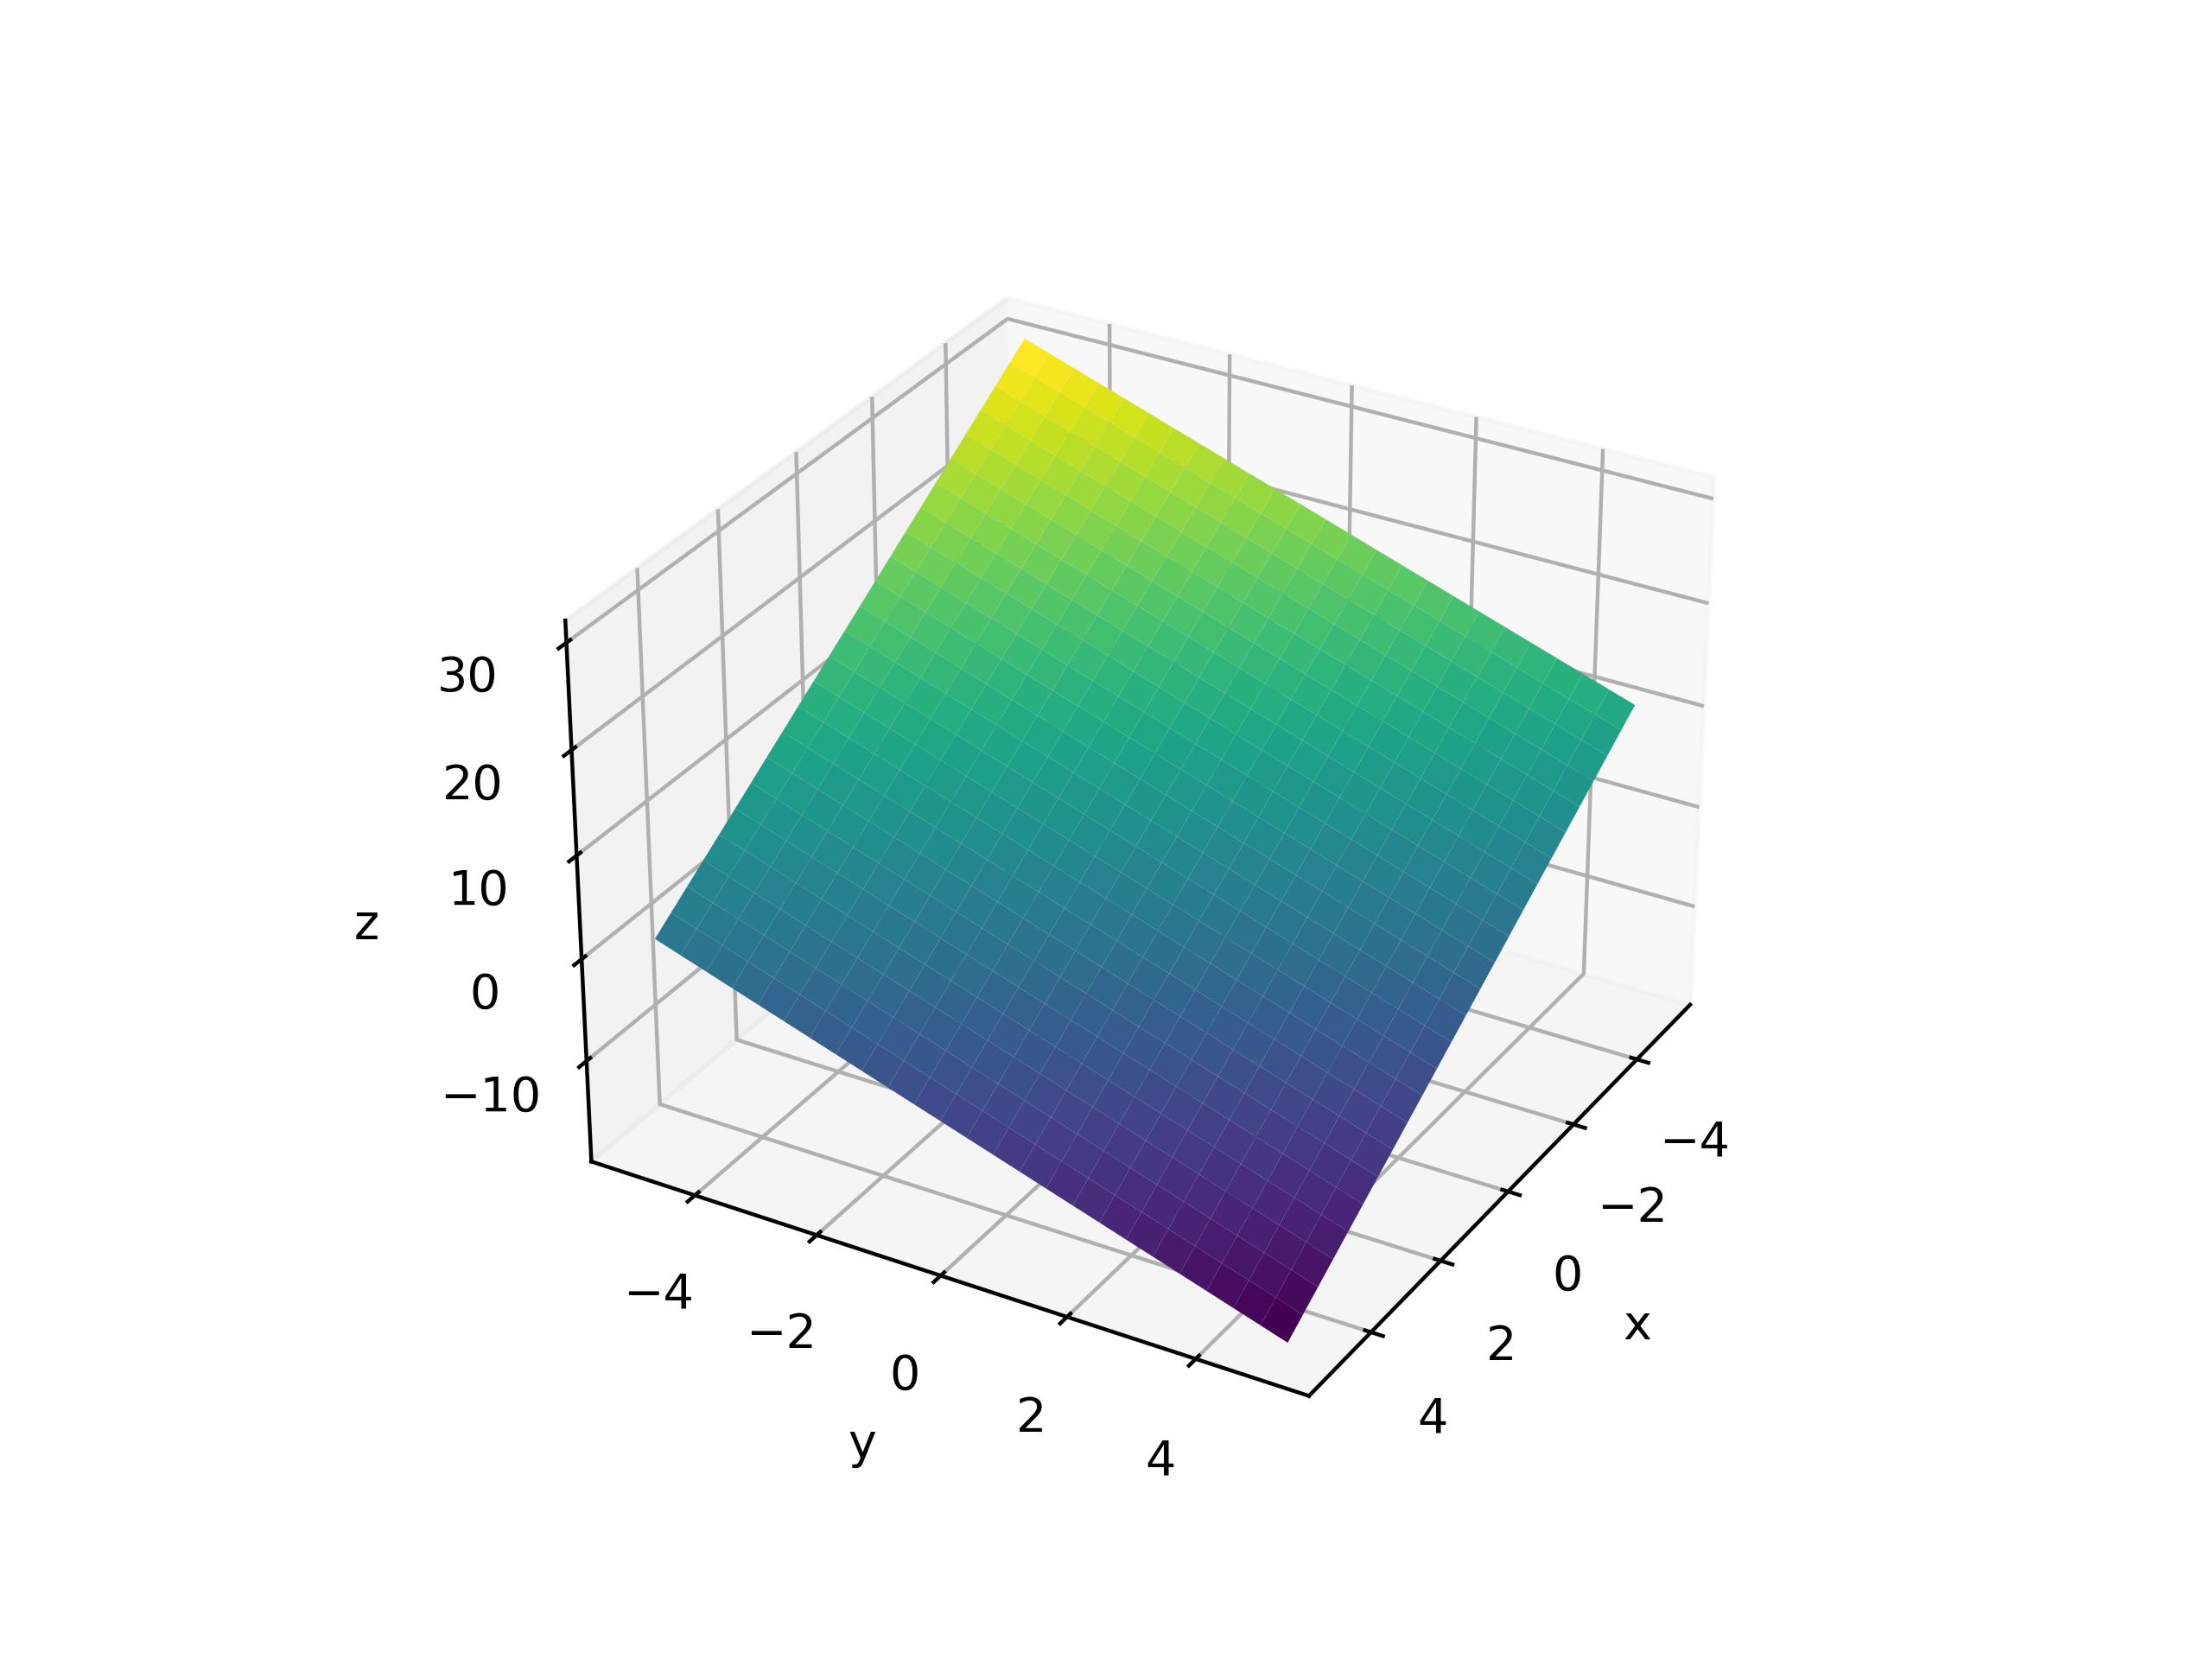
\includegraphics[scale=0.7]{figuras/grafico1.png}
\end{center}
\end{frame}


\subsection*{Curvas de Nível}

\begin{frame}[label=funcoes]
\frametitle{Curvas e Superfícies de Nível }
%\begin{scriptsize}

Uma curva ao longo da qual uma função $z=f(x,y)$ tem valor constante é denominada \dt{curva de nível} da função $f$.

\begin{center}
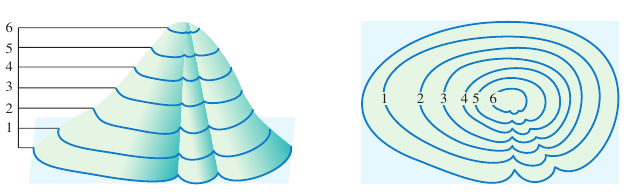
\includegraphics[scale=0.5]{figuras/nivel1.png}
\end{center}

 Quando a função $f$ representa a temperatura, as curvas de nível de $f$ são chamadas \dt{isotermas}. Se $f$ representa o potencial elétrico, as curvas de nível de $f$ são ditas \dt{curvas equipotenciais}. A equação da curva de nível ao longo da qual a função assume valor constante $k$ é
$$f(x,y)=k.$$
Se $S$ é a superfície do gráfico de uma função $f$, um conjunto de curvas de nível de uma função $f$ é dito \dt{um mapa de contorno da superfície $S$}.



%\end{scriptsize}
\end{frame}

\begin{frame}[label=funcoes]
\only<1>{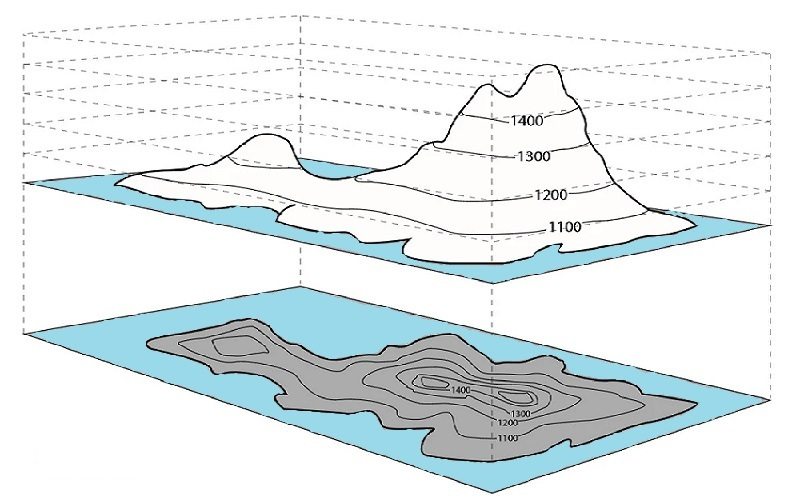
\includegraphics[scale=0.6]{figuras/nivel3.jpg}}
\end{frame}

\begin{frame}[label=funcoes]
\begin{exe}
		A temperatura em cada ponto $(x,y)$ de uma placa de metal plana é dada, em graus, pela função $T(x,y)=9x^2+4y^2$. Faça uma mapa de contorno das isotermas.
\end{exe}
\end{frame}



\begin{frame}[label=funcoes]
\begin{center}

\only<1>{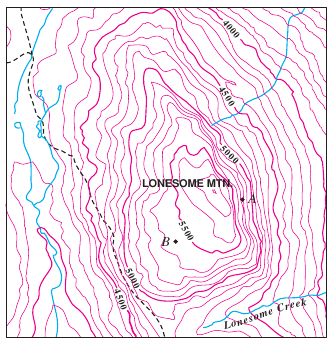
\includegraphics[scale=0.9]{figuras/nivel2.png}

Mapa topográfico de uma região montanhosa.
}
\only<2>{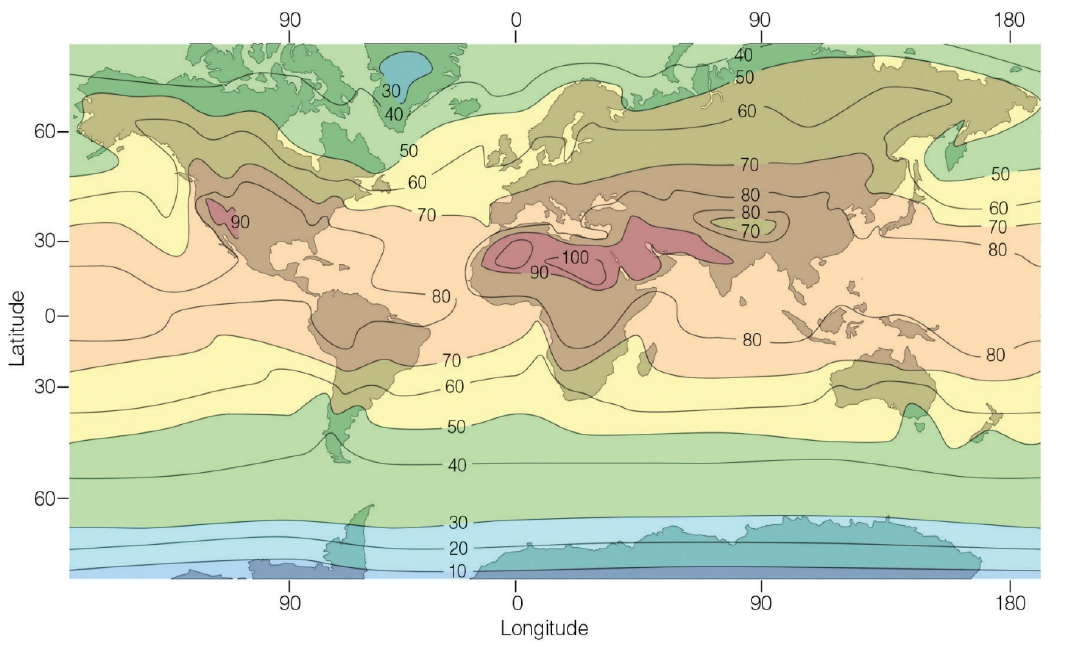
\includegraphics[scale=0.4]{figuras/nivel3.png}

Temperatura média do ar ao nível do mar no mês de julho em Fahrenheit}
\only<3>{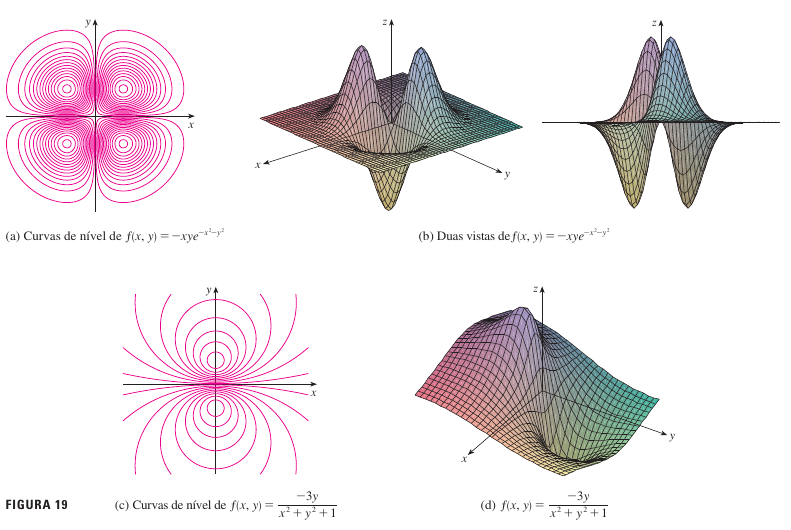
\includegraphics[scale=0.6]{figuras/nivel4.png}}
\only<4>{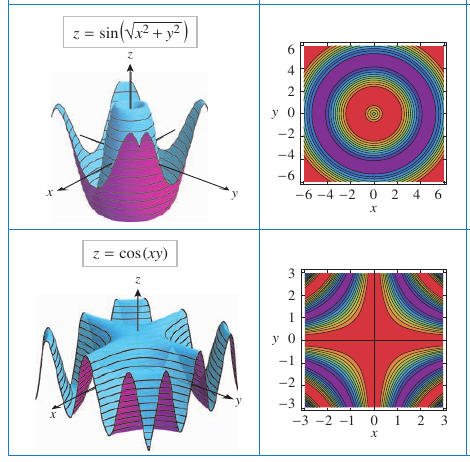
\includegraphics[scale=0.6]{figuras/nivel5.png}

Degradê de cores para indicar os níveis. Varia do roxo para o vermelho na ordem crescente.
}
\only<5>{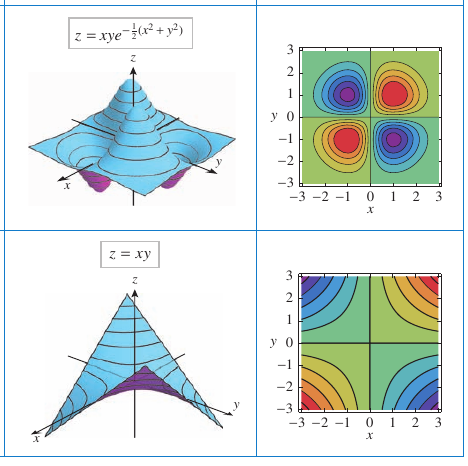
\includegraphics[scale=0.7]{figuras/nivel6.png}}
\end{center}
\end{frame}




\subsection*{Superfícies de Nível}
\begin{frame}[label=funcoes]
\frametitle{Superfícies de Nível}
%\begin{scriptsize}
\uncover<1->{ No caso de funções de três variáveis, um conjunto no qual uma função $f(x,y,z)$ tem valor constante é dita \dt{uma superfície de nível} da função $f$.

\begin{exe} Descreva as superfícies de nível da função $f(x,y,z)=x^2+y^2+z^2$.
\end{exe}}

\begin{center}
	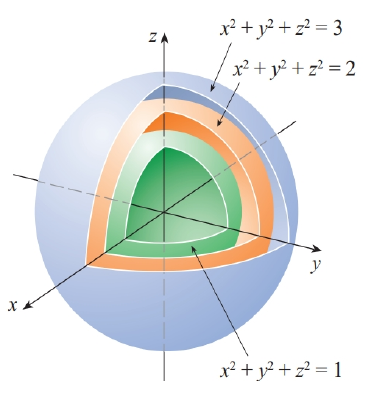
\includegraphics[scale=0.5]{figuras/nivel-superfice.png}
\end{center}

%\end{scriptsize}
\end{frame}


\begin{frame}[label=funcoes]
\begin{casa}
\begin{enumerate}
\item Esboce a região de domínio da função 
\[f(x,y)=x\log(y^2-x)\]
\item Determine o domínio e esboce o gráfico da função  $f(x,y)=\sqrt{9-x^2-y^2}$.

\item Faça um mapa de contorno da função $f(x,y)=4-x^2-y$ para os níveis $5,4,3,2,1,0,-1$ e faça um esboço do gráfico.

\item Descreva as superfícies de nível da função $f(x,y,z)=z-x^2-y^2$.
\end{enumerate}
\end{casa}
\end{frame}
